\subsection{Deep Learning}
El Deep Learning ha transformado el campo del procesamiento de imágenes al permitir la automatización de tareas complejas como la clasificación, detección de objetos y segmentación de imágenes. Las redes neuronales profundas, particularmente las redes neuronales convolucionales (CNNs), son la arquitectura principal utilizada para el análisis de imágenes debido a su capacidad para capturar características espaciales jerárquicas en los datos visuales.


\begin{figure}[h]
    \centering
    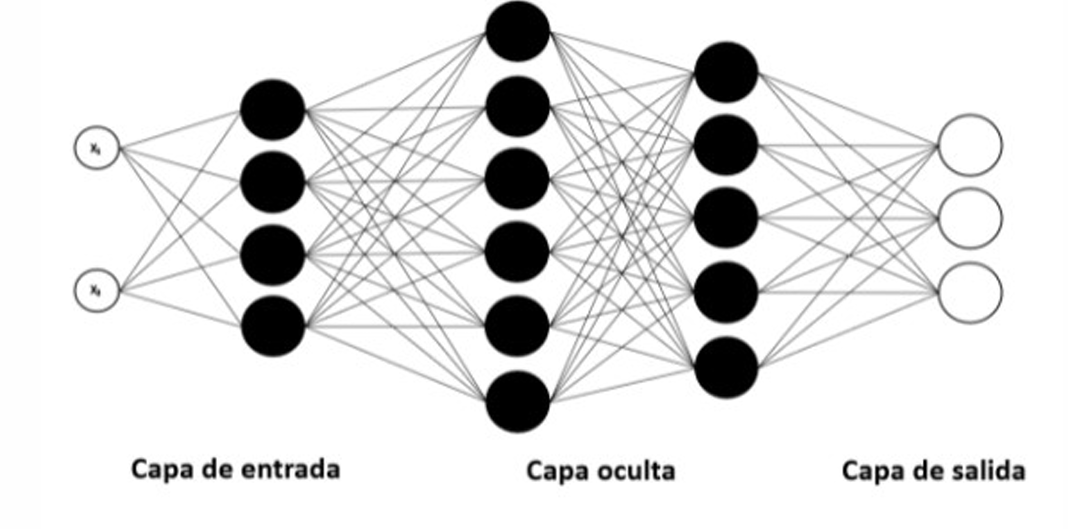
\includegraphics[width=0.5\textwidth]{2/figures/Redes neuronales.png}
    \caption{Metodología}
    \label{fig:etiqueta_de_la_figura}
\end{figure}

\subsubsection{Redes Neuronales Convolucionales (CNNs)}
Las Redes Neuronales Convolucionales (CNNs, por sus siglas en inglés) son una clase de redes neuronales diseñadas específicamente para procesar datos con una estructura de cuadrícula, como las imágenes. Una CNN consta de varias capas que aprenden automáticamente las características relevantes de las imágenes a medida que se entrenan:

\begin{itemize}
    \item \textbf{Capa Convolucional}: Aplica filtros (o kernels) a la imagen para extraer características locales como bordes, texturas y patrones. Cada filtro se mueve a través de la imagen generando un mapa de características. Para una imagen de entrada \(X\), el resultado de aplicar un filtro \(K\) es un mapa de características \(F\) dado por:

    \[
    F(i,j) = \sum_m \sum_n X(i+m,j+n) \cdot K(m,n),
    \]

    donde \(m\) y \(n\) son los índices de los elementos del filtro \(K\), y \(i, j\) son los índices de los píxeles en la imagen.

    \item \textbf{Capa de Pooling}: Reduce la dimensionalidad de las características extraídas al resumir pequeñas regiones de las imágenes (por ejemplo, mediante el \textit{max-pooling}, que selecciona el valor máximo en cada región). Esto ayuda a reducir el número de parámetros y a controlar el sobreajuste.
\end{itemize}



\subsection{Clustering}
Es una técnica de aprendizaje no supervisado que agrupa un conjunto de datos en subconjuntos llamados \textit{clusters}, de manera que los objetos dentro de un mismo cluster sean más similares entre sí que con los de otros clusters. Es una herramienta clave en la minería de datos, el análisis de datos y el aprendizaje automático.

A diferencia del aprendizaje supervisado, donde se dispone de etiquetas de clase, el clustering busca encontrar estructuras ocultas en los datos sin conocimiento previo de las etiquetas.

\subsection{Clustering de Imágenes}
El clustering de imágenes es una técnica que agrupa imágenes en clusters basados en la similitud de sus características. La idea es que las imágenes dentro de un mismo cluster sean más similares entre sí que con las de otros clusters. Este proceso involucra varios pasos, desde la extracción de características hasta la evaluación de la calidad del clustering.

\subsubsection{Preprocesamiento de Imágenes}
Antes de aplicar el clustering a imágenes, es fundamental realizar un preprocesamiento que generalmente incluye:

\begin{itemize}
    \item \textbf{Extracción de Características}: Las imágenes se transforman en vectores de características que describen aspectos relevantes de su contenido. Algunos métodos comunes incluyen:
        \begin{itemize}
            \item \textbf{SIFT (Scale-Invariant Feature Transform)}: Extrae características clave invariantes a escala y rotación.
            \item \textbf{HOG (Histogram of Oriented Gradients)}: Captura la distribución de gradientes en una imagen.
            \item \textbf{Redes Neuronales Convolucionales (CNNs)}: Extraen características profundas que capturan detalles complejos en las imágenes.
        \end{itemize}
    \item \textbf{Reducción de Dimensionalidad}: Las características extraídas pueden ser de alta dimensión, por lo que se utilizan técnicas como PCA (Principal Component Analysis) o t-SNE (t-Distributed Stochastic Neighbor Embedding) para reducir la dimensión y facilitar el clustering.
\end{itemize}

\subsection{K-means}
Su objetivo es dividir un conjunto de datos en \(k\) grupos o \textit{clusters}, minimizando la varianza dentro de cada grupo. La esencia de K-means es encontrar \(k\) centroides, uno para cada cluster, de manera que los puntos de datos dentro de un cluster estén más cerca de su propio centroide que de cualquier otro.

Dado un conjunto de datos \(X = \{x_1, x_2, \dots, x_n\}\) donde cada \(x_i \in \mathbb{R}^d\), el algoritmo K-means intenta particionar los datos en \(k\) clusters \(C = \{C_1, C_2, \dots, C_k\}\), tal que se minimice el criterio de suma de los cuadrados de las distancias (SSE, \textit{Sum of Squared Errors}) entre los puntos y sus respectivos centroides.

La función objetivo que el algoritmo K-means intenta minimizar es la siguiente:

\[
J(C) = \sum_{i=1}^{k} \sum_{x_j \in C_i} \| x_j - \mu_i \|^2,
\]

donde:
\begin{itemize}
    \item \(C_i\) es el \(i\)-ésimo cluster,
    \item \(\mu_i = \frac{1}{|C_i|} \sum_{x_j \in C_i} x_j\) es el centroide del cluster \(C_i\), calculado como el promedio de los puntos de datos asignados a ese cluster,
    \item \(\| x_j - \mu_i \|\) es la distancia Euclidiana entre un punto \(x_j\) y el centroide \(\mu_i\).
\end{itemize}

Esta función mide la compacidad de los clusters. El objetivo del algoritmo es minimizar \(J(C)\), es decir, minimizar la suma de las distancias al cuadrado entre los puntos de datos y sus centroides correspondientes.


